\documentclass[12pt]{article}
\usepackage{graphicx}
\usepackage{fullpage}
\usepackage{verbatim}
\usepackage{caption}
\usepackage{float}
\usepackage[nottoc]{tocbibind} 
\usepackage{appendix}
\usepackage{titlesec}
\usepackage{tikz}
\usepackage{listings}
\usepackage{hyperref}
\hypersetup{
    colorlinks=true,
    linkcolor=blue,
    filecolor=magenta,      
    urlcolor=blue,
}
\usepackage[utf8]{inputenc}
\urlstyle{same}
\usetikzlibrary{shapes,arrows}
\titleformat{\chapter}[display]
  {\normalfont\bfseries}{}{0pt}{\Large}
  \usepackage[T1]{fontenc}
\usepackage[utf8]{inputenc}

  


\begin{document}
  \begin{titlepage}
    \begin{center}
      \begin{Large}
      \textbf{ Assignment- 9\\
       \vspace*{0.5cm}
       ELP - 718 Telecom Software Laboratory\\
       \vspace{1cm}
       Ch Krishna Chaitanya\\
       2019JTM2674\\
       2019-21\\}
      \end{Large}
       \vspace{1cm}
      {\Large  A report on Python with OOPs concepts}
       \vfill
       \begin{figure}[h!]
          \centering
          
\includegraphics{iitdelhi.png}
       \end{figure}
       \vfill
      \begin{Large}
      \textbf{ Bharti School of \\
       Telecommunication Technology and Management\\
       IIT Delhi\\
       India\\
      }\end{Large}
       \medskip
       \today
    \end{center}
    \vfill
  \end{titlepage}
  
  \tableofcontents
  
  \clearpage
  \section*{Objective Statement}
   To test our understanding of object oriented concepts using python.

  \section{Problem Statement -1}
 To ceate class named Author which holds data members: name (string), email (string), and gender 

  \subsection{Problem Satement}
  
  \subsection{Algorithm and Implementation}
  \begin{itemize}
  \item Create Class Author
  \item Initialise constructor with attribures name, gender, email
  \item Name and Gender cannot be changed hence only getters
  \item Email can be updated or changed using setter function
  \item Implement print method in Author class
  \item Display details using print method in Author class
  \end{itemize}
  \subsection{Flowchart}
    % Define block styles
  \tikzstyle{decision} = [diamond, draw, fill=blue!20, 
    text width=4.5em, text badly centered, node distance=3cm, inner sep=0pt]
\tikzstyle{block} = [rectangle, draw, fill=blue!20, 
    text width=6em, text centered, rounded corners, minimum height=4.5em,node distance=2.2cm]
\tikzstyle{line} = [draw, -latex']
\tikzstyle{cloud} = [draw, ellipse,fill=red!20, node distance=3cm,
    minimum height=3em]
  \begin{center}    
\begin{tikzpicture}[node distance = 2cm, auto]
    % Place nodes
    
    \node [cloud] (init) {start};
    \node [block, below of=init] (First) {Create Author class};
    \node [block, below of=First] (Second) {Initialise name, gender, email};
    \node [block, below of=Second] (Third) {Create name, gender, email getters};
    \node [block, below of=Third] (Fourth) {Create setter for email};
    \node [block, below of=Fourth] (Fifth) {Display Information};
    \node [block, below of=Fifth] (Sixth) {Stop};
 
    
    
    % Draw edges
    \path [line] (init) -- (First);
    \path [line] (First) -- (Second);
    \path [line] (Second) -- (Third);
     \path [line] (Third) -- (Fourth);
    \path [line] (Fourth) -- (Fifth);
    \path [line] (Fifth) -- (Sixth);
  
   
    
\end{tikzpicture}
\end{center}
  \subsection{Input and Output format}
  \subsubsection{Input Format} 
Create object with Author Class\\


\subsubsection{Output Format}
Peter Jones (m) at peter@somewhere.com

  \subsection{Test Cases}
  \subsubsection{Input1}
 person1=Author("Krishna","kc@gmail.com","m")\\

    
  \subsubsection{Output1}
 Krishna (m) at kc@gmail.com\\

\subsection{Screenshots}

\includegraphics[width=\linewidth]{lab9_2.png}
\newpage
  \section{Problem Statement -2}
  \subsection{Problem Satement}
    To make an application to handle the students results using classes in python 



  \subsection{Algorithm and Implementation}
  \begin{itemize}
  \item Login panel for student and admin should be created
  \item Validate password for admin
  \item If user is student, display his marks
  \item If user is admin, three options are available
  \item Display required data based on option chosen
  \item Check if he wants to exit or continue
  \end{itemize}
  \subsection{Flowchart}
    % Define block styles
\tikzstyle{decision} = [diamond, draw, fill=blue!20, 
    text width=4.5em, text badly centered, node distance=3cm, inner sep=0pt]
\tikzstyle{block} = [rectangle, draw, fill=blue!20, 
    text width=6.5em, text centered, rounded corners, minimum height=3em]
\tikzstyle{line} = [draw, -latex']
\tikzstyle{cloud} = [draw, ellipse,fill=red!20, node distance=3cm,
    minimum height=3em]
\begin{center}    
\begin{tikzpicture}[node distance = 2cm, auto]
    % Place nodes
    
    \node [cloud] (init) {start};
    \node [block, below of=init] (First) {Display login panel};
    \node [block, below of=First] (Second) {Enter Username};
    \node [decision, below of=Second] (decide) {Check Admin or student};
     \node [block, below of=decide,node distance=3cm] (Staff) {Display student marks};
     \node [block, left of=decide,node distance=4cm] (Customer) {Select 1.Add user\\
2.Update marks\\
3.Display marks};
     
    \node [block, below of=Customer,node distance=3cm] (cust_des) {Display selected option};
    \node [block, below of=cust_des] (stop_cust) {stop};
    \node [block, below of=Staff] (stop_st) {stop};
  
    
    % Draw edges
    \path [line] (init) -- (First);
    \path [line] (First) -- (Second);
    \path [line] (Second) -- (decide);
     \path [line] (decide) --(Staff);
     \path [line] (Staff) --(stop_st);
     \path [line] (decide) --(Customer);
     \path [line] (Customer) --(cust_des);
     \path [line] (cust_des) --(stop_cust);
     
    
   
\end{tikzpicture}
\end{center}
  
 \newpage
  \subsection{Test Cases}
  
	\subsubsection{Input}
	Enter\\
1.Admin\\
2.Student 2\\
\subsubsection{Output}
Enter\\
1.Admin\\
2.Student 2\\
Enter Roll no 25\\
Student login succesfull\\
Total marks of student with roll no.25 is 89\\
\subsection{Screenshots}
\subsubsection{Screenshot1}
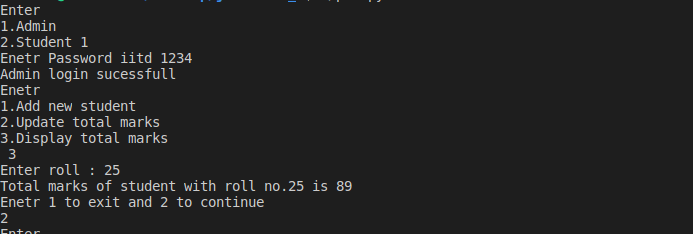
\includegraphics[width=\linewidth]{lab9_1.png}
\clearpage
\subsubsection{Screenshot2}
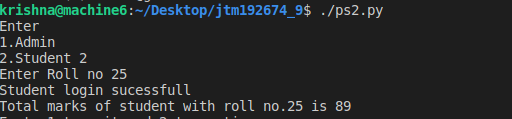
\includegraphics[width=\linewidth]{lab9_3.png}
\newpage
 \appendix
   \appendixpage
   \addappheadtotoc
  \section*{Problem 1}
  {\large \textbf{code:}}
  \verbatiminput{ps1.py}
  \section*{Problem 2}
  {\large \textbf{code:}}
  \verbatiminput{ps2.py}
  
  
\newpage
\begin{thebibliography}{11}
\bibitem{flowchart} 
Flowchart using Latex\\
Kjell Magne Fauske \\
\url{http://www.texample.net/tikz/examples/simple-flow-chart/}

\bibitem{Python Basics}
Python Basics \\
\url{https://docs.python.org/3/}

\bibitem{Python OOPS Concepts}
Python OOPS Concepts\\
\url{https://code.tutsplus.com/articles/python-from-scratch-object-oriented-programming--net-21476}

\bibitem{Git Hub}
Git Hub\\
\url{https://help.github.com/en/articles/fork-a-repo}

\bibitem{Python Getters and Setters}
Python Getters and Setters\\
\url{https://www.datacamp.com/community/tutorials/property-getters-setters}

\end{thebibliography}

   
   
\end{document}
